\documentclass[../report.tex]{subfiles} \begin{document} \paragraph*{}
Hình trạng mạng là mô hình thể hiện kết nối giữa các nút mạng với nhau thông qua các kênh truyền. Trong mỗi hệ thống cụ thể, việc lựa chọn một hình trạng mạng là yếu tố rất quan trọng do đây là yếu tố liên quan đến việc xây dựng hệ thống, lựa chọn các thiết bị chuyển tiếp trung gian có thông số phù hợp (số cổng kết nối, tốc độ xử lý và truyển tiếp gói tin ...). Không những thế, hình trạng mạng còn ảnh hưởng đến việc lựa chọn/xây dựng giải thuật định tuyến. Mỗi mô hình mạng khác nhau thường yêu cầu các thuật toán định tuyến khác nhau để có thể sử dụng được những đặc điểm riêng biệt của một mô hình mạng. Do vậy, để đánh giá một mô hình mạng mới, người ta thường quan tâm đến chi phí khi xây dựng hệ thống trên thực tế và hiệu năng mà mô hình mạng đó đem lại.

\paragraph*{}
Có hai loại hình trạng mạng: indirect network và direct network. Trong direct network, mỗi thiết bị được liên kết với một tập các thiết bị khác trong mạng. Trong trường hợp này, bất cứ sự trao đổi nào giữa hai thiết bị không phải là hàng xóm của nhau thì thông tin sẽ được chuyển qua các thiết bị trung gian trước khi đến được thiết bị đích. Thay vì kết nối trực tiếp giữa các thiết bị, trong mạng indirect network kết nối các thiết bị với nhau thông qua các switch. Nếu tồn tại nhiều switch, chúng sẽ được kết nối với nhau thông qua các liên kết điểm - điểm. Trong trường hợp này, thông tin trao đổi giữa các thiết bị đều phải thông qua một hoặc nhiều switch.

\subsection{Direct Network}
\paragraph*{}
Direct network hay point-to-point network là một kiến trúc mạng phổ biến đáp ứng tốt nhu cầu làm việc với một lượng lớn vi xử lý. Một direct network bao gồm một tập các node, mỗi node được kết nối trực tiếp tới một tập các node khác trong mạng. Mỗi node là một máy tính sở hữu các tài nguyên riêng như: vi xử lý, bộ nhớ và các thiết bị hỗ trợ khác. Các node có thể có các chức năng khác nhau. Thành phần chung của các node đó là router, có nhiệm vụ xử lý thông điệp giao tiếp giữa các node. Vì lý do đó, direct network còn được gọi là router-based network. Mỗi router có nhiều kết nối trực tiếp tới các hàng xóm của nó. Thông thường, hai node là hàng xóm của nhau được kết nối bằng một cặp kênh vô hướng và có chiều ngược nhau. Kênh hai chiều cũng có thể được dùng để kết nối hai node hâng xóm với nhau. 

\paragraph*{}
Mỗi router hỗ trợ một số lượng các kênh vào ra. Internal channel hay port dùng để kết nối router với vi xử lý/ bộ nhớ của node. Thường sẽ chỉ có một cặp internal channel, tuy nhiên để tránh hiện tượng nghẽn giao tiếp giữa các vi xử lý/ bộ nhớ với router. External channel được sử dụng cho việc giao tiếp giữa các router. Thông thường mỗi node có một số lượng cố định các kênh vào ra và mỗi kênh vào sẽ có tương ứng kênh ra ghép với nó. 

\paragraph*{}
Direct network được mô hình hóa là một đồ thị G(N, C), N đại diện cho số lượng node và C là số lượng kênh. Những thuộc tính cần quan tâm trong direct network là:
\begin{itemize}
    \item Bậc của node: số kênh mà node đang kết nối tới các hàng xóm của nó.
    \item Diameter: Khoảng cách lớn nhất trong những khoảng cách nhỏ nhất giữa các node.
    \item Regularity: Một mạng được xem là regular khi tất cả các node có cùng bậc.
    \item Symmetry: Một mạng là symmetric khi nó có dạng giống nhau khi quan sát từ mọi node.
\end{itemize}

\subsubsection{Các topo điển hình}
Các topo trong thực tế thường có cấu trúc liên kết trực giao. Mỗi node có ít nhất một liên kết với nó theo mõi chiều.
\paragraph{Lưới n chiều}
Mạng gồm $k_0$ x $k_1$ x $k_2$ x \ldots x $k_{n-2}$ x $k_{n-1}$ node, $k_i$ là số node theo dọc theo chiều i, với $k_i \ge 2$ và $0 \le i \le n - 1$. Mỗi node X được xác định bởi n tọa độ ($x_{n-1}, x_{n-2},$ \ldots, $x_1, x_0$), với $0 \le x_i \le k_i - 1$ và $0 \le i \le n - 1$. Hai node X và Y là hàng xóm khi và chỉ khi $y_i = x_i$ với mọi $0 \le i \le n - 1$, ngoại trừ một chiều j mà $y_j = x_j \pm 1$. Do đó, node sẽ có từ n tới 2n hàng xóm, điều này phụ thuộc vào vị trí của nó trên lưới. Chính vì thế, topo này không có tính \textit{regular}.
\begin{figure}[H]
    \centering
    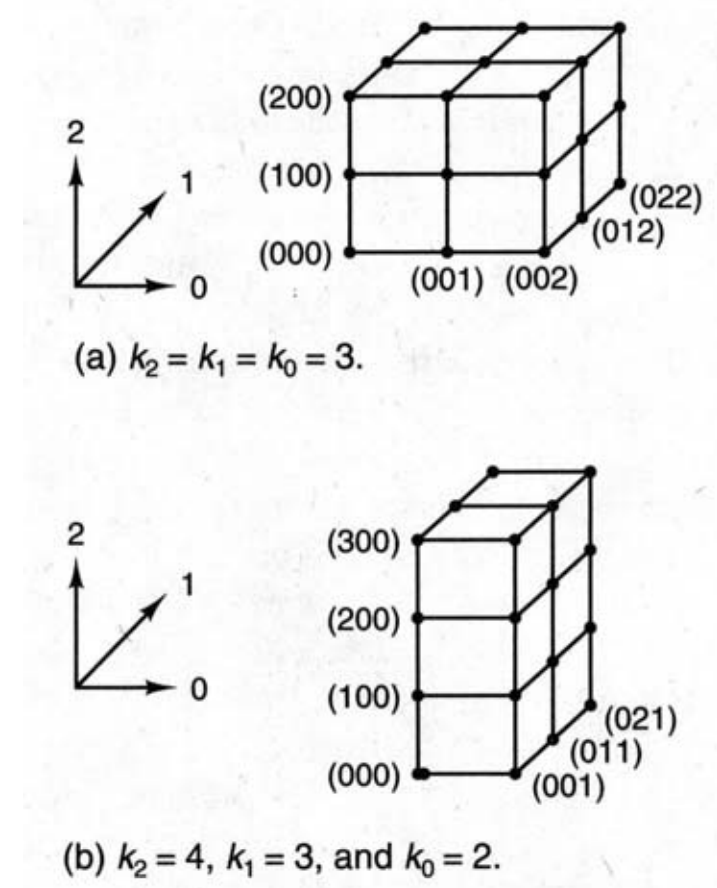
\includegraphics[width=10cm]{figures/nDim.png}
    \caption{Lưới 3 chiều}
\end{figure}

\paragraph{Mạng Torus (k-ary n-cube)}
Trong cấu trúc mạng Torus, mọi node đều có cùng số lượng hàng xóm (bậc giống nhau). Topo này khác với lưới n chiều ở chỗ số lượng node ở mõi chiều là bằng nhau và bắng k. Hai node X và Y là hàng xóm của nhau nếu và chỉ nếu $y_i = x_i$ với mọi $0 \le i \le n - 1$, ngoại trừ một chiều j mà $y_j = x_j \pm 1$ mod k. Sự khác biệt này giúp cho cấu trúc này có tính chất \textit{regular} và \textit{symmetry}. Từ đây, ta thấy node có n hàng xóm nếu k = 2 và 2n hàng xóm nếu k > 2. Khi n = 1, k-ary n-cube trở thành topo ring hai chiều với k node. Kênh truyền của mạng Torus có thể là một chiều hoặc hai chiều. 

\begin{figure}[H]
    \centering
    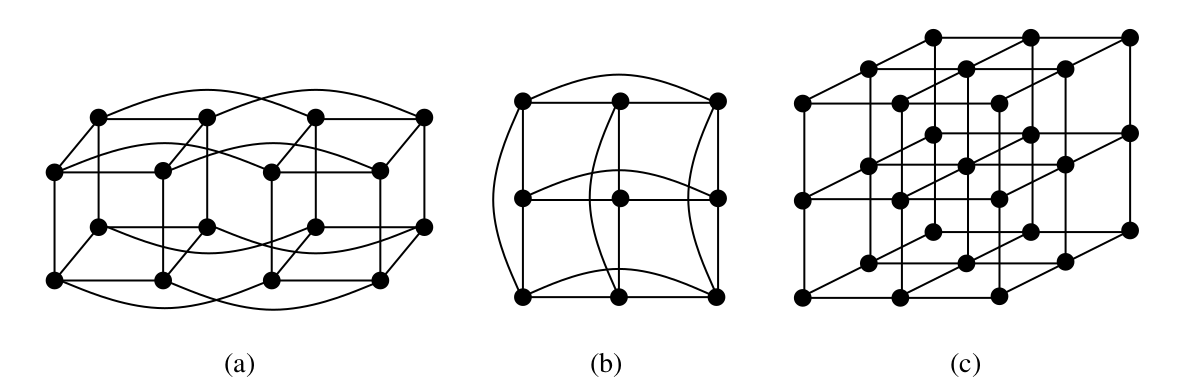
\includegraphics[width=\textwidth]{figures/direct.png}
    \caption{(a) 2-ary 4-cube (hypercube), (b) 3-ary 2-cube và (c) 3-ary 3-D mesh}
\end{figure}

\subsection{Indirect Network}
\paragraph*{}
Indirect Network hay mạng dựa trên switch là một phân lớp khác của mạng liên kết. Thay vì cung cấp trực tiếp kết nối giữa các node với nhau, các node sẽ giao tiếp với nhau thông qua switch. Mỗi node sẽ có một adapter để kết nối với switch. Mỗi switch sẽ có một tập các port, mỗi port bao gồm một liên kết đi vào và một liên kết đi ra. Một số lượng port trong switch có thể được kết nối với các vi xử lý hoặc bỏ trống, số lượng port còn lại sẽ kết nối với các switch khác để tạo nên kết nối giữa các vi xử lý. Cấu trúc liên kết giữa các switch sẽ định nghĩa nhiều loại hình trạng mạng khác nhau. 

\paragraph*{}
Indrirect Network cũng có thể được mô hình hóa dưới dạng một đồ thị G(N, C) - N là số lượng các switch, C là số lượng các liên kết một chiều hoặc hai chiều giữa các switch. Việc truyền thông điệp từ mọt node tới node khác yêu cầu phải đi các liên kết từ nguồn tới switch kết nối với nó, và liên kết giữa switch cuối cùng trên đường đi và node đích. Bởi vậy khoảng cách giữa hai node là khoảng cách giữa các switch kết nối trực tiếp đến những node đó cộng thêm hai đơn vị. Tương tự vậy, diamerter sẽ là khoảng cách lớn nhất giữa hai switch kết nối với một số node cộng thêm hai đơn vị. 

\begin{figure}[H]
    \centering
    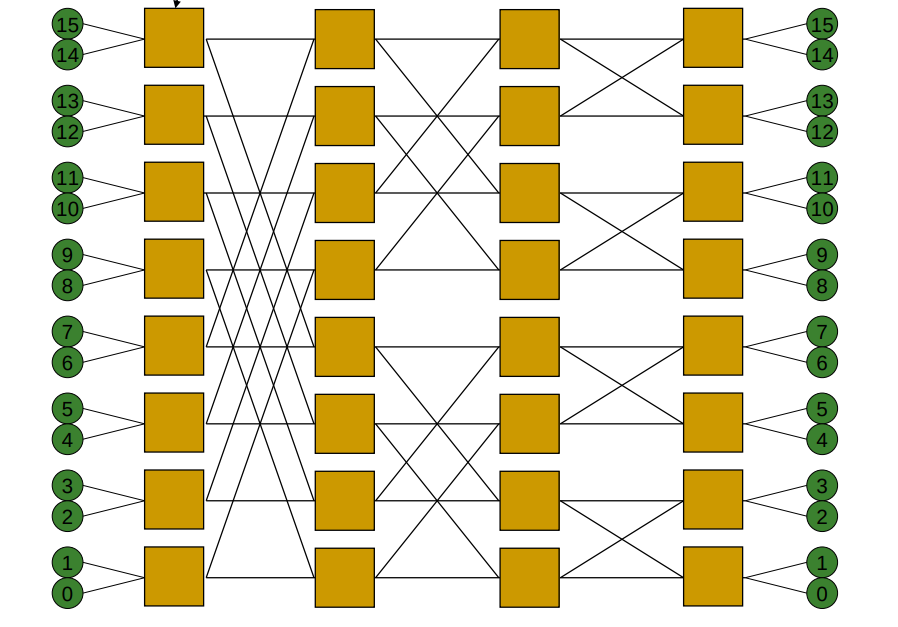
\includegraphics[width=\textwidth]{figures/indirect.png}
    \caption{Indirect network với 2 đầu vào và 2 đầu ra}
\end{figure}
\end{document}

